% Beamer template
% Author: Ozgur Taylan TURAN
% Delft University of Technology

\documentclass[aspectratio=169]{beamer}
% PACKAGES
\usepackage[english]{babel}
\usepackage{graphicx}
\usepackage{animate}
%\usepackage{calc}
\usepackage{calligra}
\usepackage[absolute,overlay]{textpos}
\usepackage[T1]{fontenc}
%\usefonttheme{serif}
\usefonttheme{professionalfonts}
\usepackage{amsmath}
\usepackage{palatino}
\usepackage{mathpazo}
\usepackage{graphicx}
%\usepackage{subfig}
\usepackage{tikz}
\usetikzlibrary{shapes,arrows}
\usepackage{xcolor}
\usepackage[T1]{fontenc}
%\usefonttheme{serif}
%\usepackage{titling}
\usepackage{graphicx}
%\usepackage{subfig}
%\usepackage{tikz}
%\usetikzlibrary{shapes,arrows}
\usepackage{mathtools}
\usepackage{cancel}
% CUSTOM PACKAGES

\usepackage{/home/taylanot/texmf/tex/beamerthemetot}
\input{/home/taylanot/texmf/presentation/tune.tex}


 % COVER PAGE INFO   
\newcommand{\mytitle}{\color{White}\huge{\textbf{BNAIC/BeNeLearn 2022}}}
\newcommand{\mysubtitle}{\color{Pink}\Large{\textbf{When MAML Learns Quickly, Does It Generalize Well?}}}
\newcommand{\myauthor}{\color{White}\textcalligra{\LARGE Ozgur Taylan Turan}}
\newcommand{\authorlabel}{\small}
\author{\authorlabel}
\setlength\bibitemsep{0.3cm} % space between entries in the reference list
\renewcommand{\bibfont}{\normalfont\scriptsize}
\renewcommand{\cite}[1]{\footnote<.->[frame]{\fullcite{#1}}}
\setbeamertemplate{bibliography item}{}
\bibliography{/home/taylanot/Dropbox/archieve_bib/mylibrary.bib}

\newcommand{\inst}[1]{$^\text{#1}$}
\newcommand{\authors}{O. Taylan Turan\inst{1}, 
David M.J. Tax\inst{1}, and 
Marco Loog\inst{1}}

\renewcommand{\institute}{\small{$^\text{1}$ Delft University of Technology, Pattern Recognition and Bioinformatics Laboratory}}

%\newcommand{\ali}{ali}
\begin{document}
% COVER PAGE

{
\def\beamer@entrycode{\vspace*{-\headheight}}
\setbeamertemplate{frametitle}[default][center]
\usebackgroundtemplate{\includegraphics[width=\paperwidth,height=\paperheight]{cover/coverart.pdf}}

\begin{frame}[plain] 

\begin{minipage}{\textwidth}
	\centering{\mytitle} \\
	\vspace{1cm}
	\centering{\color{White}\today} \\
	\vspace{1cm}
	\centering{\myauthor}\\
\end{minipage}


\end{frame}
}
\begin{frame}

  \vspace{1cm}

	\centering

	\mysubtitle

  \vspace{1cm}

  \authors
  
  \vspace{3cm}

  \institute

\end{frame}

% Outline 
%\begin{frame}{Outline}
%  \begin{itemize}
%    \item Introduction (Meta-Learning \& MAML)
%    \item Experimental Setup
%    \item (Some) Results
%    \item Conclusions
%  \end{itemize}
%\end{frame}

\section{Introduction}
% Meta-Learning
\begin{frame}{Meta-Learning}
  \begin{minipage}{0.5\textwidth}
    \begin{itemize}
      \item Introduced in 90s
      \item Leverage different learning problems for a target problem
      \item Especially useful in few-shot learning
    \end{itemize}
  \end{minipage}%
  \begin{minipage}{0.5\textwidth}
    \centering
    \includegraphics[width=\textwidth]{figures/meta_learning}
  \end{minipage}
\end{frame}

% MAML
\begin{frame}{How Does MAML\cite{finn2017} Work?}
  \only<1-5>
  {
  \begin{minipage}{0.5\textwidth}
    \begin{itemize}
      \item<1> Assume you have task distribution $p_{\mathcal{T}}$
      \item<2> Sample a batch of tasks $\{\mathcal{T}_i\}_{i=1}^M$
      \item<3> Provide an initialization for model parameters
      \item<4> Get a target task $\mathcal{T}_\text{target}$ 
      \item<5> Adaptation to a target task with limited gradient steps (quick adaptation)
    \end{itemize}
  \end{minipage}%
  \begin{minipage}{0.5\textwidth}
    \centering
    \includegraphics[width=\textwidth]{figures/maml}
  \end{minipage}
  }
\end{frame}

% What is the Problem?
\begin{frame}{What is the problem?}
\begin{minipage}{0.5\textwidth}
  \begin{itemize}
    \item Generalization 
    \item Quick adaptation is not needed by many settings
    \item Robotics/image classification/regression applications
  \end{itemize}
\end{minipage}%
\begin{minipage}{0.5\textwidth}
  \centering
  \includegraphics[width=\textwidth]{figures/generalization}
\end{minipage}
\end{frame}


% Aim
\begin{frame}{AIM}
  \centering
    \color{Pink} Investigate the effect of gradient step limitation on generalization performance!
\end{frame}    

\section{Experimental Setup}
% Experimental Setup
\begin{frame}{Experimental Setup}
  \only<1>
  {
  \begin{minipage}{\textwidth}
    \begin{itemize}
      \item Tasks: linear/nonlinear regression problems with noisy ($\varepsilon  \sim \mathcal{N}(0, \sigma^2)$) observations of functions $f(\mathbf{x})$
      \begin{equation}\label{eq:task}
    \mathbf{y}= f(\mathbf{x})+\varepsilon
  \end{equation}  
    \end{itemize}
  \end{minipage}
  \begin{minipage}{\textwidth}
    \begin{minipage}{0.5\textwidth}
      \centering
      \includegraphics[width=0.7\textwidth]{figures/lin_maml}

    $f(\mathbf{x}):=\mathbf{x}^\text{T}\mathbf{a}$
    \end{minipage}%
    \begin{minipage}{0.5\textwidth}
      \centering
      \includegraphics[width=0.7\textwidth]{figures/nonlin_maml}

    $f(\mathbf{x}):=\text{sin}(\mathbf{x}+\boldsymbol{\phi})^{\text{T}}\mathbf{a}$
    \end{minipage}
  \end{minipage}
  }
  \only<2>
  {
  \begin{minipage}{\textwidth}
    \begin{minipage}{0.5\textwidth}
      \centering
      \includegraphics[width=0.7\textwidth]{figures/lin_maml}

    $f(\mathbf{x}):=\mathbf{x}^\text{T}\mathbf{a}$


    $\mathbf{a} \sim \mathcal{N}(m\mathbf{1}, c\mathbf{I})$
    \end{minipage}%
    \begin{minipage}{0.5\textwidth}
      \centering
      \includegraphics[width=0.7\textwidth]{figures/nonlin_maml}

    $f(\mathbf{x}):=\text{sin}(\mathbf{x}+\boldsymbol{\phi})^{\text{T}}\mathbf{a}$

   
    $\mathbf{a} \sim \mathcal{N}(\mathbf{1}, c_1\mathbf{I})$


    $\boldsymbol{\phi} \sim \mathcal{N}(\mathbf{0}, c_2\mathbf{I})$

    \end{minipage}
  \end{minipage}
  }
  \only<3>
  {
    \begin{itemize}
      \item Estimator: model $\hat{M}$ trained  with a given dataset $\mathcal{Z}:=\{\mathbf{x}_i, y_i\}_{i=0}^{N}$
      \item Performance: expected error over the task distribution $p_\mathcal{T}$ and data distribution $p_\mathcal{Z}$
      \begin{equation}\label{eq:ee}
    \mathcal{E}:= \iiint(\mathcal{\hat{M}}(\mathbf{x}) - y)^2 p(\mathbf{x}, y)p_{\mathcal{Z}} p_{\mathcal{T}} d\mathbf{x} dy d\mathcal{Z} d\mathcal{T}
      \end{equation}
    \end{itemize}
  }
  \only<4>
  {
    Models under investigation;
    \begin{itemize}
      \item Linear and Kernel Ridge Regression
      \item MAML (initialized from $\mathbf{w}_\text{meta}$) with limited adaptation 
      \item Randomly initialized gradient descent 
    \end{itemize}
  }
\end{frame}

\section{Results}
% Results
\begin{frame}{(Some) Results}
\only<1>
  {
    \begin{itemize}
      \item Task Variance ($c$) for 1D-Linear Problem with $\sigma = 1$,
        $m = 0$, $k = 1$, $c = 1$, $n_{iter} = 1$ and $N=1, 10, 50$ % Add here other default values
    \end{itemize}
    \centering
    \begin{minipage}{0.3\textwidth}
      \includegraphics[width=\textwidth]{figures/lin_c_1}    
    \end{minipage}%
    \begin{minipage}{0.3\textwidth}
      \includegraphics[width=\textwidth]{figures/lin_c_2}    
    \end{minipage}%
    \begin{minipage}{0.3\textwidth}
      \includegraphics[width=\textwidth]{figures/lin_c_3}    
    \end{minipage}
  }
\only<2>
  {
    \begin{itemize}
      \item What is happening?
    \end{itemize}
    \centering
    
\includegraphics[width=0.5\textwidth]{figures/testvstrain}
  }
\only<3>
  {
    \begin{itemize}
      \item Task Variance ($c_2$) for 1D-Nonlinear Problem with $\sigma = 1$,
        $k = 1$, $c_1 = 2$, $n_{iter} = 10$ $N=1, 10, 50$ % Add here other default values
        
    \end{itemize}
    \centering
    \begin{minipage}{0.3\textwidth}
      \includegraphics[width=\textwidth]{figures/nonlin_c_1}    
    \end{minipage}%
    \begin{minipage}{0.3\textwidth}
      \includegraphics[width=\textwidth]{figures/nonlin_c_2}    
    \end{minipage}%
    \begin{minipage}{0.3\textwidth}
      \includegraphics[width=\textwidth]{figures/nonlin_c_3}    
    \end{minipage}
  }
\end{frame}

\section{Conclusions}
% Conclusions
\begin{frame}{Conclusions}
  \begin{itemize}
    \item A single-task learner can outperform MAML with limited gradient step adaptation in expectation.
    \item Small task variance is crucial for MAML performance in expectation.
    \item A similar study for supervised benchmark datasets can be done to understand the generalization performance of MAML and its variants better.
  \end{itemize}
\end{frame}

%\begin{frame}
%  \begin{minipage}{0.5\textwidth}
%    \centering
%    \color{Pink} Thanks for your attention!
%  \end{minipage}%
%  \begin{minipage}{0.5\textwidth}
%    
\includegraphics[width=0.9\textwidth]{figures/qrlogo.pdf}
%  \end{minipage}
%
%\end{frame}

\begin{frame}
  \centering
  \color{Pink} Thanks for your attention!
\end{frame}

\end{document}
